%% LyX 2.3.4.2 created this file.  For more info, see http://www.lyx.org/.
%% Do not edit unless you really know what you are doing.
\documentclass[english,dvipsnames,aspectratio=169]{beamer}
\usepackage{mathptmx}
\usepackage{eulervm}
\usepackage[T1]{fontenc}
\usepackage[latin9]{inputenc}
\usepackage{babel}
\usepackage{amstext}
\usepackage{amssymb}
\usepackage{graphicx}
\usepackage{ifthen}
\usepackage{xcolor}
\usepackage{xspace}
\usepackage{tikz}
\usetikzlibrary{tikzmark}
\usetikzlibrary{calc}
\usepackage{pgfplots}
%\pgfplotsset{compat=1.17}
\usepackage{booktabs}
\usepackage{xpatch}
\usepackage{bbm}

\xpatchcmd{\itemize}
  {\def\makelabel}
  {\ifnum\@itemdepth=1\relax
     \setlength\itemsep{2ex}% separation for first level
   \else
     \ifnum\@itemdepth=2\relax
       \setlength\itemsep{1ex}% separation for second level
     \else
       \ifnum\@itemdepth=3\relax
         \setlength\itemsep{0.5ex}% separation for third level
   \fi\fi\fi\def\makelabel
  }
 {}
 {}

\ifx\hypersetup\undefined
  \AtBeginDocument{%
    \hypersetup{unicode=true,pdfusetitle,
 bookmarks=true,bookmarksnumbered=false,bookmarksopen=false,
 breaklinks=false,pdfborder={0 0 0},pdfborderstyle={},backref=false,colorlinks=true,
 allcolors=NYUPurple,urlcolor=LightPurple}
  }
\else
  \hypersetup{unicode=true,pdfusetitle,
 bookmarks=true,bookmarksnumbered=false,bookmarksopen=false,
 breaklinks=false,pdfborder={0 0 0},pdfborderstyle={},backref=false,colorlinks=true,
 allcolors=NYUPurple,urlcolor=LightPurple}
\fi

\makeatletter

%%%%%%%%%%%%%%%%%%%%%%%%%%%%%% LyX specific LaTeX commands.
%% Because html converters don't know tabularnewline
\providecommand{\tabularnewline}{\\}

%%%%%%%%%%%%%%%%%%%%%%%%%%%%%% Textclass specific LaTeX commands.
% this default might be overridden by plain title style
\newcommand\makebeamertitle{\frame{\maketitle}}%
% (ERT) argument for the TOC
\AtBeginDocument{%
  \let\origtableofcontents=\tableofcontents
  \def\tableofcontents{\@ifnextchar[{\origtableofcontents}{\gobbletableofcontents}}
  \def\gobbletableofcontents#1{\origtableofcontents}
}

%%%%%%%%%%%%%%%%%%%%%%%%%%%%%% User specified LaTeX commands.
\usetheme{CambridgeUS} 
\beamertemplatenavigationsymbolsempty


% Set Color ==============================
\definecolor{NYUPurple}{RGB}{87,6,140}
\definecolor{LightPurple}{RGB}{165,11,255}


\setbeamercolor{title}{fg=NYUPurple}
\setbeamercolor{frametitle}{fg=NYUPurple}

\setbeamercolor{background canvas}{fg=NYUPurple, bg=white}
\setbeamercolor{background}{fg=black, bg=NYUPurple}

\setbeamercolor{palette primary}{fg=black, bg=gray!30!white}
\setbeamercolor{palette secondary}{fg=black, bg=gray!20!white}
\setbeamercolor{palette tertiary}{fg=gray!20!white, bg=NYUPurple}

\setbeamertemplate{headline}{}
\setbeamerfont{itemize/enumerate body}{}
\setbeamerfont{itemize/enumerate subbody}{size=\normalsize}

\setbeamercolor{parttitle}{fg=NYUPurple}
\setbeamercolor{sectiontitle}{fg=NYUPurple}
\setbeamercolor{sectionname}{fg=NYUPurple}
\setbeamercolor{section page}{fg=NYUPurple}
%\setbeamercolor{description item}{fg=NYUPurple}
%\setbeamercolor{block title}{fg=NYUPurple}

\setbeamertemplate{blocks}[rounded][shadow=false]
\setbeamercolor{block body}{bg=normal text.bg!90!NYUPurple}
\setbeamercolor{block title}{bg=NYUPurple!30, fg=NYUPurple}



\AtBeginSection[]{
  \begin{frame}
  \vfill
  \centering
\setbeamercolor{section title}{fg=NYUPurple}
 \begin{beamercolorbox}[sep=8pt,center,shadow=true,rounded=true]{title}
    \usebeamerfont{title}\usebeamercolor[fg]{title}\insertsectionhead\par%
  \end{beamercolorbox}
  \vfill
  \end{frame}
}

\makeatother

\setlength{\parskip}{\medskipamount} 

\input ../macros

\begin{document}
\input ../rosenberg-macros

\title[CSCI-GA 2565]{Introduction to Machine Learning}
\author{Mengye Ren}
\date{September 3, 2024}
\institute{NYU}

\makebeamertitle
\mode<article>{Just in article version}

\begin{frame}{Contents}
\tableofcontents{}
\end{frame}

\begin{frame}{Logistics}
\begin{itemize}
\item Class webpage: \url{https://nyu-cs2565.github.io/2024-fall} 
\begin{itemize}
    \item Course materials (lecture slides, homeworks) will be made available on the website
\end{itemize}
\item Discussion / questions on CampusWire: \url{https://campuswire.com/p/G4788841F} \\
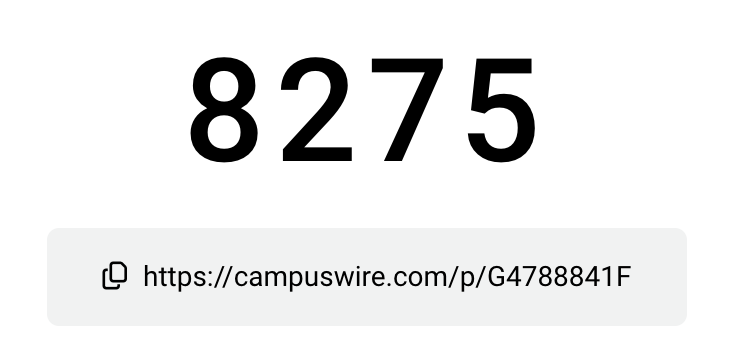
\includegraphics[width=0.4\textwidth,trim={0 0 0 0},clip]{figures/campuswire.png}
% \url{https://campuswire.com/p/G74AFD6C8}
\item Sign up to Gradescope to submit homework assignments (entry code \textbf{Z3PB2W})
\end{itemize}
\begin{itemize}
\item Office Hour: Thursday 1:00-2:00 pm, Room 508, 60 Fifth Ave.
\end{itemize}
\end{frame}

\section{Logistics}

\begin{frame}{Course Staff}
\begin{itemize}
\item Instructor:
    \begin{itemize}
        \item Mengye Ren (\texttt{mr3182@nyu.edu})
    \end{itemize}

\item Graders:
    \begin{itemize}
        \item Pavan Ravishankar (\texttt{pr2248@nyu.edu})
        \item Yilun Kuang ({\texttt{yk2516@nyu.edu}})
    \end{itemize}
\item All course material, assignment, and exam related questions should be posted on CampusWire.
\item Assignment regrade requests should be initiated on Gradescope. Further questions directed to the graders.
\item I will only respond to administration related emails.
\end{itemize}
\end{frame}

\begin{frame}{Assessment}
\begin{itemize}
\item 4 assignments ($40\%$)
% \begin{itemize}
\item Midterm Exam (Oct 22) ($30\%$)
\item Final Project ($30\%$)
\item Extra credits ($2\%$) answer other students' questions in a substantial and helpful way on Campuswire
\end{itemize}
\end{frame}
%
\begin{frame}{Homework}
\begin{itemize}
    \item Submit through Gradescope as a \textbf{PDF document}
    \item Late policy: You have 4 late days in total which can be used throughout the semester without penalty (see more details on website).

\item You can discuss with other students on the homework assignments, but:
\begin{itemize}
\item Write up the solutions and code on your own;
\item List the names of the students you discussed with.
\end{itemize}
\item If your solution or code is substantially similar to other students then the incident will be reported to the University.

\end{itemize}
\end{frame}

\begin{frame}{Final Project}
\begin{itemize}
\item Groups of 3 students (by Oct 22, after the midterm).
\item Goals:
\begin{itemize}
\item Find a problem and a dataset
\item Survey existing approaches, identify remaining challenges
\item Apply and design ML algorithms in real applications
\item Compare and analyze empirical performance
\end{itemize}
\item Project proposal due Oct 29, 2024, 12PM (Noon)
\item Last lecture: Project presentation
\item Final report due Wednesday, Dec 13, 2024, 12PM (Noon)
\end{itemize}
\end{frame}

\begin{frame}{Prerequisites}
\begin{itemize}
\item Multivariate Calculus: partial derivatives/gradient.
\item Linear Algebra: vector/matrix manipulations, properties.
\item Probability Theory: common distributions; Bayes Rule.
\item Statistics: expectation, variance, covariance, median; maximum likelihood.
\item Programming: Python, numpy
\end{itemize}
\end{frame}

\section{Course Overview and Goals}
\begin{frame}{Syllabus (Tentative)}

12 weeks of instruction + 1 week midterm exam + 1 week project presentation
\begin{itemize}

\item 2 weeks: introduction to \textbf{machine learning}, \textbf{optimization}

\pause
\item 2 weeks: \textbf{Linear }methods for binary classification
and regression (also\textbf{ kernel methods)}

\pause
\item 2 weeks: \textbf{Probabilistic models}, \textbf{Bayesian}
methods

\pause
\item 2 weeks: \textbf{Multiclass} classification and introduction to \textbf{structured prediction}

\pause
\item 3 weeks: \textbf{Nonlinear} methods (\textbf{trees}, \textbf{ensemble}
methods, and \textbf{neural networks})

\pause
\item 1 week: \textbf{Unsupervised} learning: \textbf{clustering} and \textbf{latent variable} models
\end{itemize}
\end{frame}

\begin{frame}{The high level goals of the class}
\begin{itemize}
\item Our focus will be on the fundamental building blocks of machine learning
\item Understand what kind of problems can ML help solve
\pause
\item Accomodate different types of input, output, problem characteristics
\pause
\item Understand the pros \& cons of each method, understand the motivation why we choose one method over the other
\pause
\item Fancy new methods are often combination of basic techniques
\item Apply and develop ML algorithms in practical problems
\end{itemize}
\end{frame}

\begin{frame}{The level of the class}
\begin{itemize}
\item Many ML algorithms have been implemented in standard libraries (e.g. sklearn)
\item Many people only know how to call these library functions.
\item We will learn how to implement each ML algorithm \textbf{from scratch} using numpy alone, without any ML libraries.
\item Once we have implemented an algorithm from scratch once, we will use the sklearn version.
\end{itemize}
\end{frame}

\section{Introduction to Machine Learning}

\begin{frame}{What is learning?}
  \textit{ "The activity or process of gaining knowledge or skill by studying, practicing, being taught, or experiencing something."
    \begin{flushright}Merriam Webster dictionary\end{flushright}}
  \pause
  \vspace{1em}
  \textit{ ``A computer program is said to \emph{learn} from experience E with respect to some class of tasks T and performance measure P, if its performance at tasks in T, as measured by P, improves with experience E.''
  \begin{flushright}Tom Mitchell\end{flushright}}
\end{frame}

\begin{frame}{Machine learning as meta-programming}
  \begin{itemize}
  \setlength\itemsep{1em}
  \item For many problems, it's difficult to program the correct behavior by hand
    \begin{itemize}
    \item recognizing people and objects
    \item understanding human speech
    \end{itemize}
    \pause
    \item Machine learning approach: program an algorithm to automatically learn from data, or from experience, and output a program, typically to solve a prediction problem:
    \begin{itemize}
    \item Given an \textbf{input} $x$,
    \item \textbf{Predict} an \textbf{output $y$.} 
    \end{itemize}

    \pause
  \item Why might you want to use a learning algorithm?
    \pause
    \begin{itemize}
    \item hard to code up a solution by hand (e.g.~vision, speech)
    \item system needs to adapt to a changing environment (e.g.~spam detection)
    \item want the system to perform \emph{better} than the human programmers
    \end{itemize}
  \end{itemize}
\end{frame}

\begin{frame}{Example: Spam Detection}

Let's start with a few canonical examples.
\begin{itemize}
\item \textbf{Input x:} Incoming email
\end{itemize}
\begin{center}
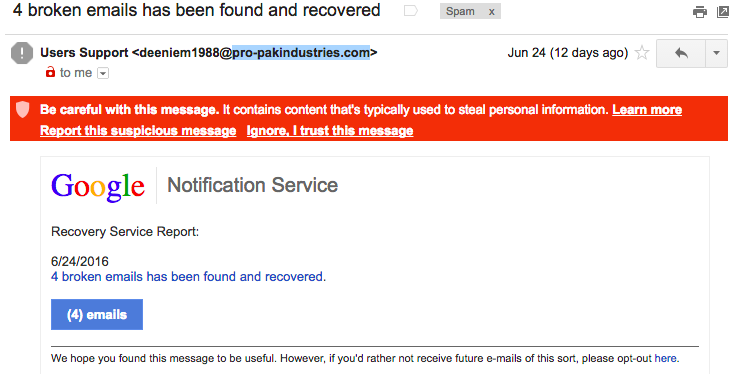
\includegraphics[width=0.6\textwidth, trim={0 6cm 0 0}, clip]{figures/spam-email}
\end{center}

\pause
\begin{itemize}
\item \textbf{Output y: }``SPAM'' or ``NOT SPAM''

\pause
\item This is a \textbf{binary classification} problem: there are two possible outputs.
\end{itemize}
\end{frame}

\begin{frame}{Example: Medical Diagnosis}
\begin{itemize}
\item \textbf{Input x:} Symptoms (fever, cough, fast breathing, shaking, nausea, ...)
\pause

\item \textbf{Output y:} Diagnosis (pneumonia, flu, common cold, bronchitis, ...)

\pause
\item A \textbf{multiclass classification} problem: choosing an output out of a \emph{discrete} set of possible outputs.
\end{itemize}

\pause
How do we express uncertainty about the output?
\begin{itemize}
\item \textbf{Probabilistic classification} or \textbf{soft classification}:
\begin{eqnarray*}
\text{\ensuremath{\pr}(pneumonia)} & = & 0.7\\
\text{\ensuremath{\pr}(flu)} & = & 0.2\\
\vdots &  & \vdots
\end{eqnarray*}
\end{itemize}
\end{frame}

\begin{frame}{Example: Predicting a Stock Price}
\begin{itemize}
\item \textbf{Input x:} History of the stock's prices
\pause
\item \textbf{Output y:} The price of the stock at the close of the next day
\end{itemize}

\pause
\begin{itemize}
    \item This is called a \textbf{regression} problem (for historical reasons): the output is \emph{continuous}.
\end{itemize}

\end{frame}

\begin{frame}{Comparison to Rule-Based Approaches (Expert Systems)}
% \begin{itemize}
Consider the problem of medical diagnosis.

\begin{enumerate}
    \item Talk to experts (in this case, medical doctors).
    \item Understand how the experts come up with a diagnosis.
    \pause
    \item Implement this process as an algorithm (a \textbf{rule-based system}): e.g., a set of symptoms $\rightarrow$ a particular diagnosis.
    \pause
    \item Use logical deduction to infer new rules from the rules that are stored in the knowledge base.  
\end{enumerate}
% \end{itemize}
\end{frame}

\begin{frame}{Rule-Based Approach}
\begin{center}
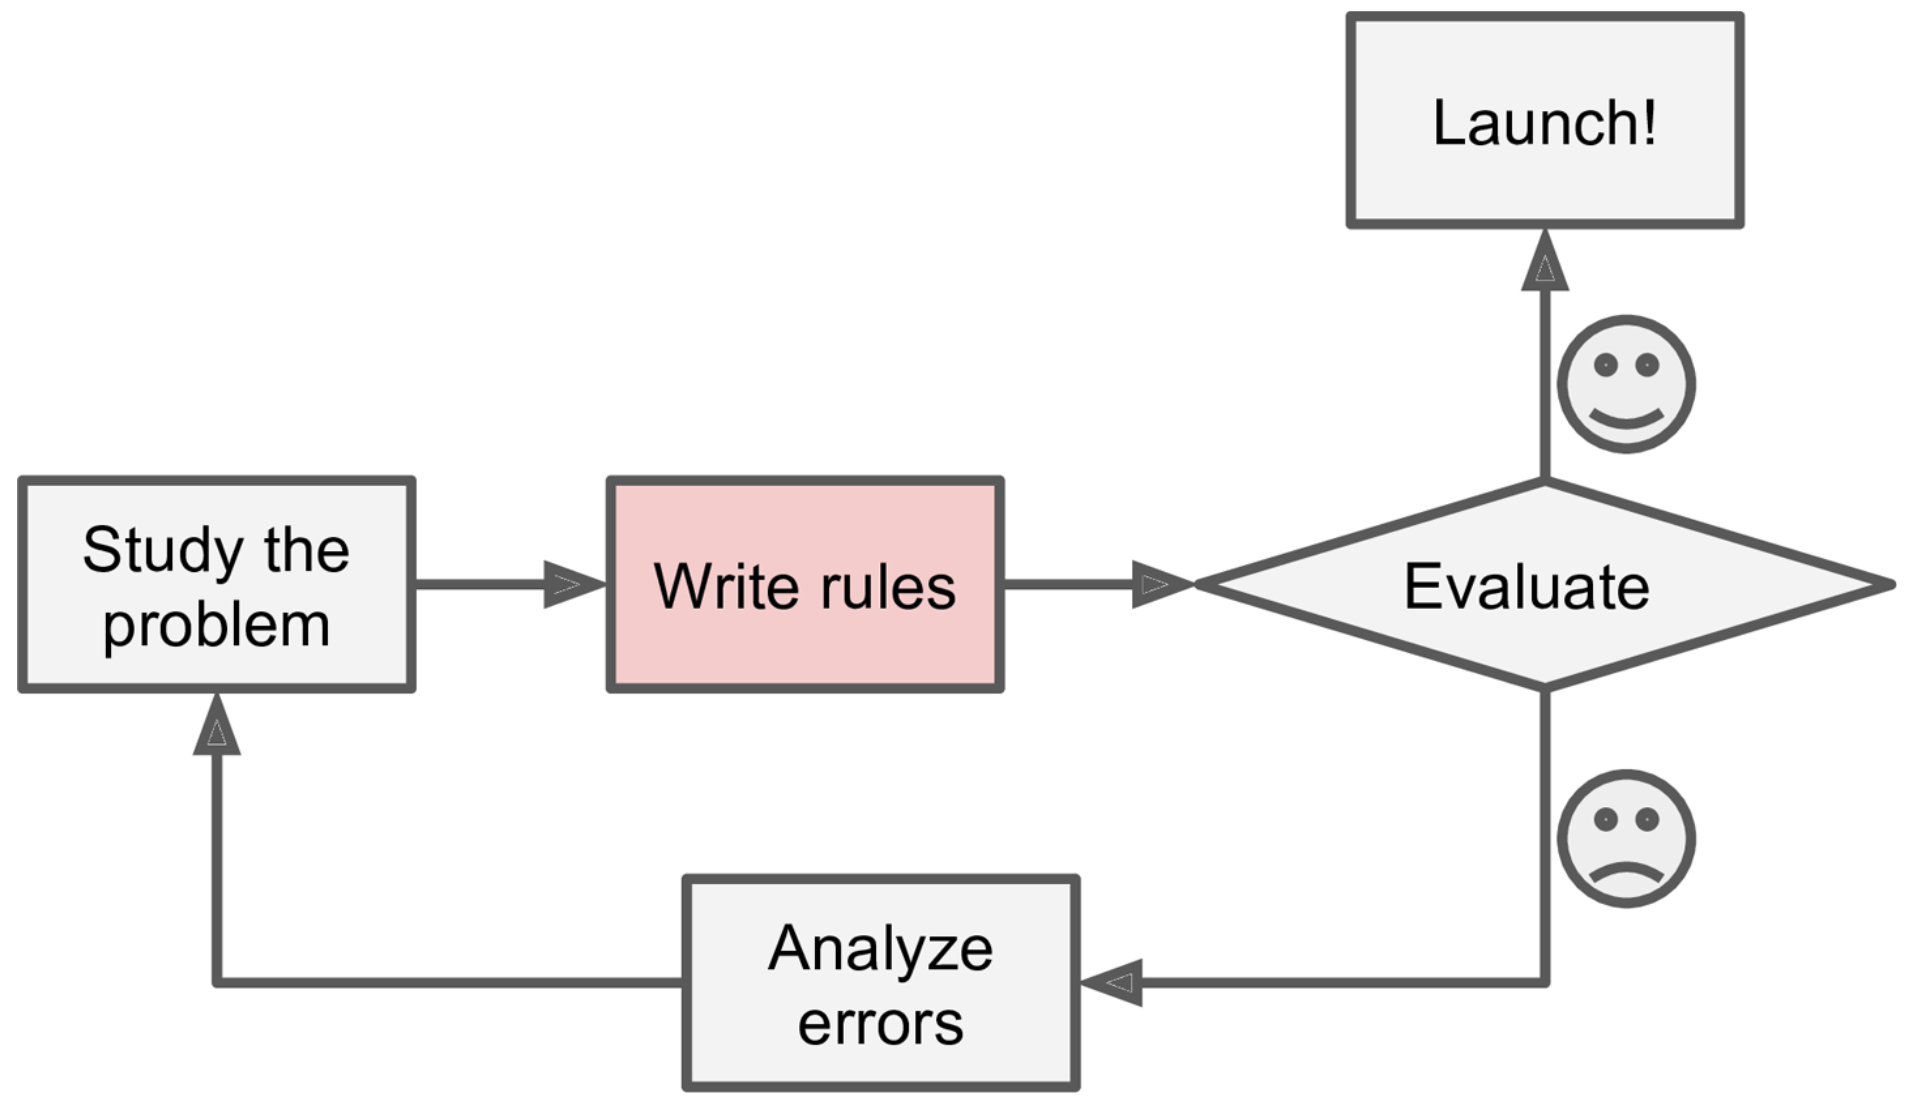
\includegraphics[height=0.7\textheight]{figures/geron-fig1-1}\let\thefootnote\relax\footnotetext{\tiny{Fig 1-1 from \emph{Hands-On Machine Learning with Scikit-Learn and TensorFlow} by Aurelien Geron (2017).}}
\par\end{center}
\end{frame}

\begin{frame}{Advantages of Rule-Based Approaches}
\begin{itemize}
    \item Leverage existing domain expertise.
    \pause
    \item Generally \textbf{interpretable}: We can describe the rule to another human
    \pause
    \item Produce reliable answers for the scenarios that are included in the knowledge bases.
\end{itemize}
\end{frame}

\begin{frame}{Limitations of Rule-Based Systems}

\begin{itemize}
\item Labor intensive to build: experts' time is expensive.
\pause
\item Rules work very well for areas they cover, but often do not \textbf{generalize} to unanticipated input combinations.
\pause
\item Don't naturally handle uncertainty.
\end{itemize}
\end{frame}

\begin{frame}{The Machine Learning Approach}
\begin{itemize}
    \item Instead of explicitly engineering the process that a human expert would use to make the decision...

    \item We have the machine \textbf{learn} on its own from inputs and outputs (decisions).

    \pause
    \item We provide \textbf{training data}:
    many examples of (input $x$, output $y$) pairs, e.g.

\begin{itemize}
\item A set of videos, and whether or not each has a cat in it.
\item A set of emails, and whether or not each one should go to the spam folder.
\end{itemize}

\item Learning from training data of this form (inputs and outputs) is called \textbf{supervised learning}.
\end{itemize}
\end{frame}

\begin{frame}{Machine Learning Algorithm}
\begin{itemize}
\item A \textbf{machine learning algorithm} learns from the training data:
\begin{itemize}
\item \textbf{Input}: Training Data (e.g., emails $x$ and their labels $y$)
\item \textbf{Output}: A prediction function that produces output
$y$ given input $x$.
\end{itemize}

\item The goal of machine learning is to find the ``best'' (to be defined) prediction function \textbf{automatically, based on the training data}

\pause

\item The success of ML depends on
    \begin{itemize}
        \item The availability of large amounts of data;
        \item \textbf{Generalization} to unseen samples (the test set): just memorizing the training set will not be useful.
    \end{itemize}
\end{itemize}
\end{frame}

\begin{frame}{Machine Learning Approach}
\begin{center}
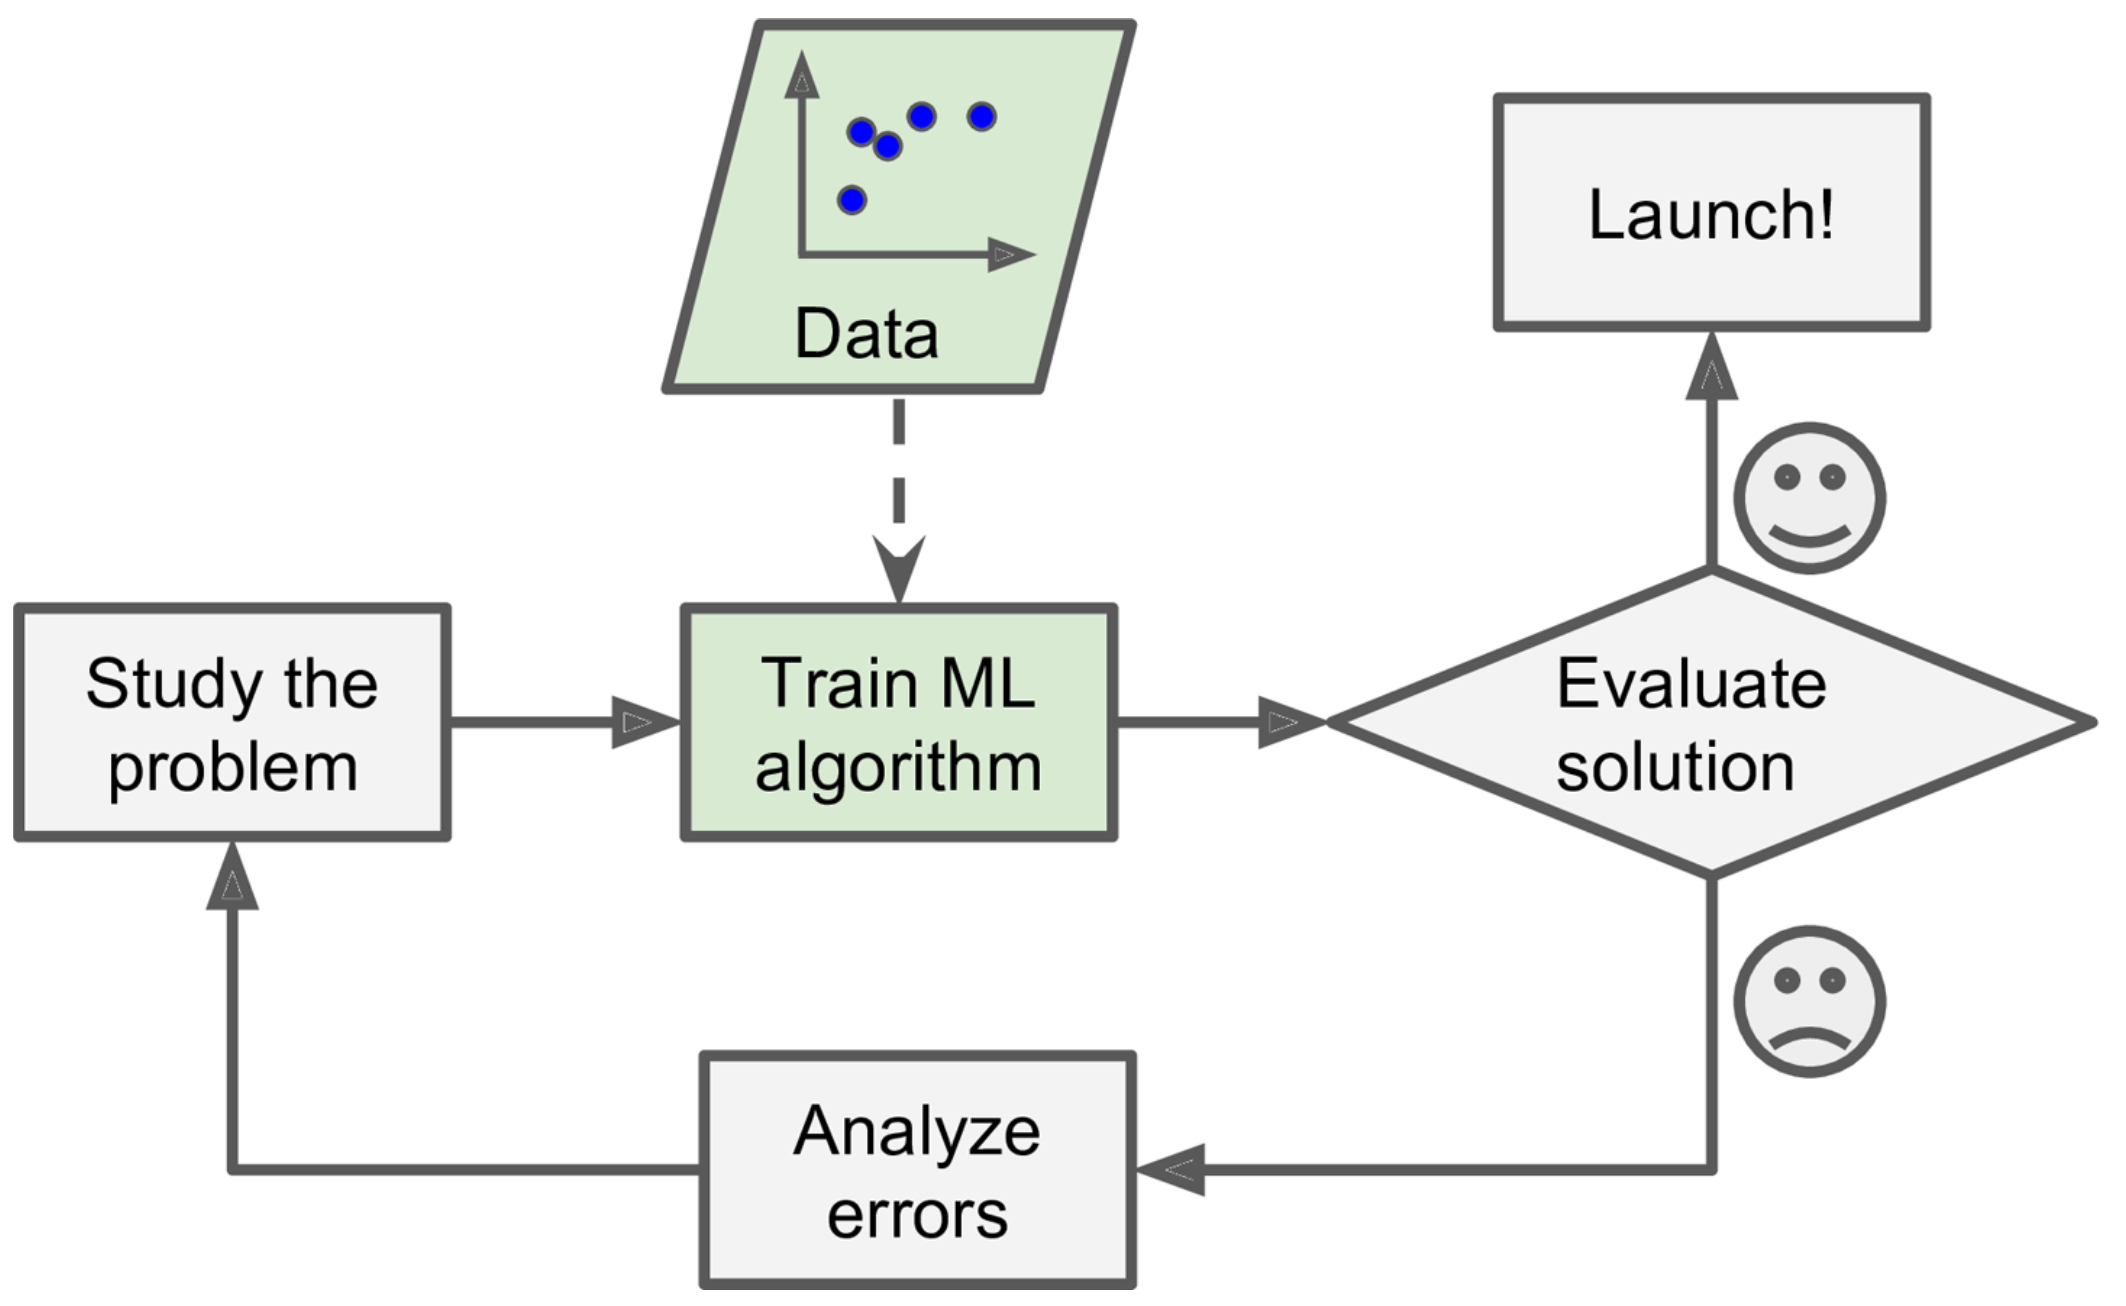
\includegraphics[height=0.7\textheight]{figures/geron-fig1-2}
\par\end{center}

\mode<article>{We've swapped out rule writing with ``machine learning.'' But how
does adjust the ML training process by analyzing errors?}
\begin{center}
\let\thefootnote\relax\footnotetext{\tiny{Fig 1-2 from \emph{Hands-On Machine Learning with Scikit-Learn and TensorFlow} by Aurelien Geron (2017).}}
\par\end{center}

\end{frame}

\begin{frame}{Key concepts}
    \begin{itemize}[<+->]
    \item The most common \textbf{ML problem types}:

\begin{itemize}
    \item Classification (binary and multiclass)
\item Regression
\end{itemize}

\item \textbf{Prediction function}: predicts output $y$ (e.g. spam or not?) given input $x$ (e.g. email)
\item \textbf{Training data}: a set of (input $x$, output $y$) pairs
\item \textbf{Supervised learning algorithm}: takes training data and produces a prediction function
\item Beyond prediction
    \begin{itemize}
        \item \textbf{Unsupervised learning}: finding structures in data, e.g. clustering
        \item \textbf{Reinforcement learning}: optimizing long-term objective, e.g. Go  
        \item \textbf{Representation learning}: learning good features of real-world objects, e.g. text
    \end{itemize}
\end{itemize}
\end{frame}

\begin{frame}
    {Core Questions in Machine Learning}
    Given any task, the following questions need to be answered:
    \begin{itemize}
        \item \textbf{Modeling}: What class of prediction functions are we considering?
        \pause
        \item \textbf{Learning}: How do we learn the ``best'' prediction function in this class from our training data?
        \pause
        \item \textbf{Inference}: How do we compute the output of the prediction function for a new input?
    \end{itemize}
\end{frame}

\begin{frame}{Relations to statistics}
  \begin{itemize}
  \setlength\itemsep{1em}
  \item It's similar to statistics...
    \begin{itemize}
    \item Both fields try to uncover patterns in data
    \item Both fields draw heavily on calculus, probability, and linear algebra, and share many of the same core algorithms
    \end{itemize}
    \pause
  \item But it's not statistics...
    \begin{itemize}
    \item Stats is more concerned with \textbf{helping scientists and policymakers} draw good conclusions; ML is more concerned with \textbf{building autonomous agents}
    \item Stats puts more emphasis on \textbf{interpretability and mathematical rigor}; ML puts more emphasis on predictive \textbf{performance, scalability, and autonomy}
    \end{itemize}
  \end{itemize}
\end{frame}

\begin{frame}{Relations to AI}
  \begin{itemize}
    \setlength\itemsep{1em}
    \item Nowadays, ``machine learning'' is often brought up with ``artificial intelligence'' (AI)
    \pause
    \item AI does not often imply a learning based system
      \begin{itemize}
        \item Symbolic reasoning
        \item Rule based system
        \item Tree search
        \item etc.
      \end{itemize}
    \pause
    \item Learning based system $\rightarrow$ learned based on the data $\rightarrow$ more flexibility, good at solving pattern recognition problems.
  \end{itemize}
\end{frame}

\begin{frame}{Relations to human learning}
  \begin{itemize}
    \setlength\itemsep{1em}
    \item It is tempting to imagine machine learning as a component in AI just like human learning in ourselves.
    \pause
    \item Human learning is:
      \begin{itemize}
        \item Very data efficient
        \item An entire multitasking system (vision, language, motor control, etc.)
        \item Flexible to adapt new skills
        \item Takes at least a few years :)
      \end{itemize}
    \item For serving specific purposes, machine learning doesn't have to look like human learning in the end.
    \pause
    \item Machines may borrow ideas from biological systems (e.g. neural networks).
    % \pause
    % \item There may also be biological constraints.
  \end{itemize}
\end{frame}

\begin{frame}{History of machine learning}
  \begin{itemize}
    \item 1957 --- Perceptron algorithm (implemented as a circuit!)
    % The New York Times reported the perceptron to be "the embryo of an electronic computer that [the Navy] expects will be able to walk, talk, see, write, reproduce itself and be conscious of its existence."
    \item 1959 --- Arthur Samuel wrote a learning-based checkers program that could defeat him
    \item 1969 --- Minsky and Papert's book \emph{Perceptrons} (limitations of linear models)
    \pause
  \item 1980s --- Some foundational ideas
    \begin{itemize}
    \item Connectionist psychologists explored neural models of cognition
    \item 1984 --- Leslie Valiant formalized the problem of learning as PAC learning
    \item 1988 --- Backpropagation (re-)discovered by Geoffrey Hinton and colleagues
    \item 1988 --- Judea Pearl's book \emph{Probabilistic Reasoning in Intelligent Systems} introduced Bayesian networks
    \end{itemize}
  \item 1990s --- the ``AI Winter'', a time of pessimism and low funding
    \pause
  \end{itemize}
\end{frame}

\begin{frame}{History of machine learning}
  \begin{itemize}
  \item A lot of practical ML algorithms were invented in the 90s: CNNs, SVMs, boosting, etc.
    % \begin{itemize}
    % \item Markov chain Monte Carlo, variational inference, kernels and support vector machines, boosting, convolutional networks
    % \end{itemize}
    \pause
  \item 2000s --- applied AI fields (vision, NLP, etc.) adopted ML
    \pause
  \item 2010s --- deep learning
    \begin{itemize}
    \item 2010--2012 --- neural nets smashed records in speech-to-text and object recognition
    \pause
    \item Increasing adoption by the tech industry, many downstream problems
    \pause
    \item 2014 --- GANs and generative AI
    \pause
    \item 2016 --- AlphaGo defeated the human Go champion
    \pause
    \item 2018--2020 --- AlphaFold predicts protein structure
    \pause
    \item 2022 --- ChatGPT, chatbot, general intelligence
    \end{itemize}
  \end{itemize}
\end{frame}

\begin{frame}{History of machine learning}
  Top ML conferences attendance over year:
  % \vspace{1em}
  \begin{center}
    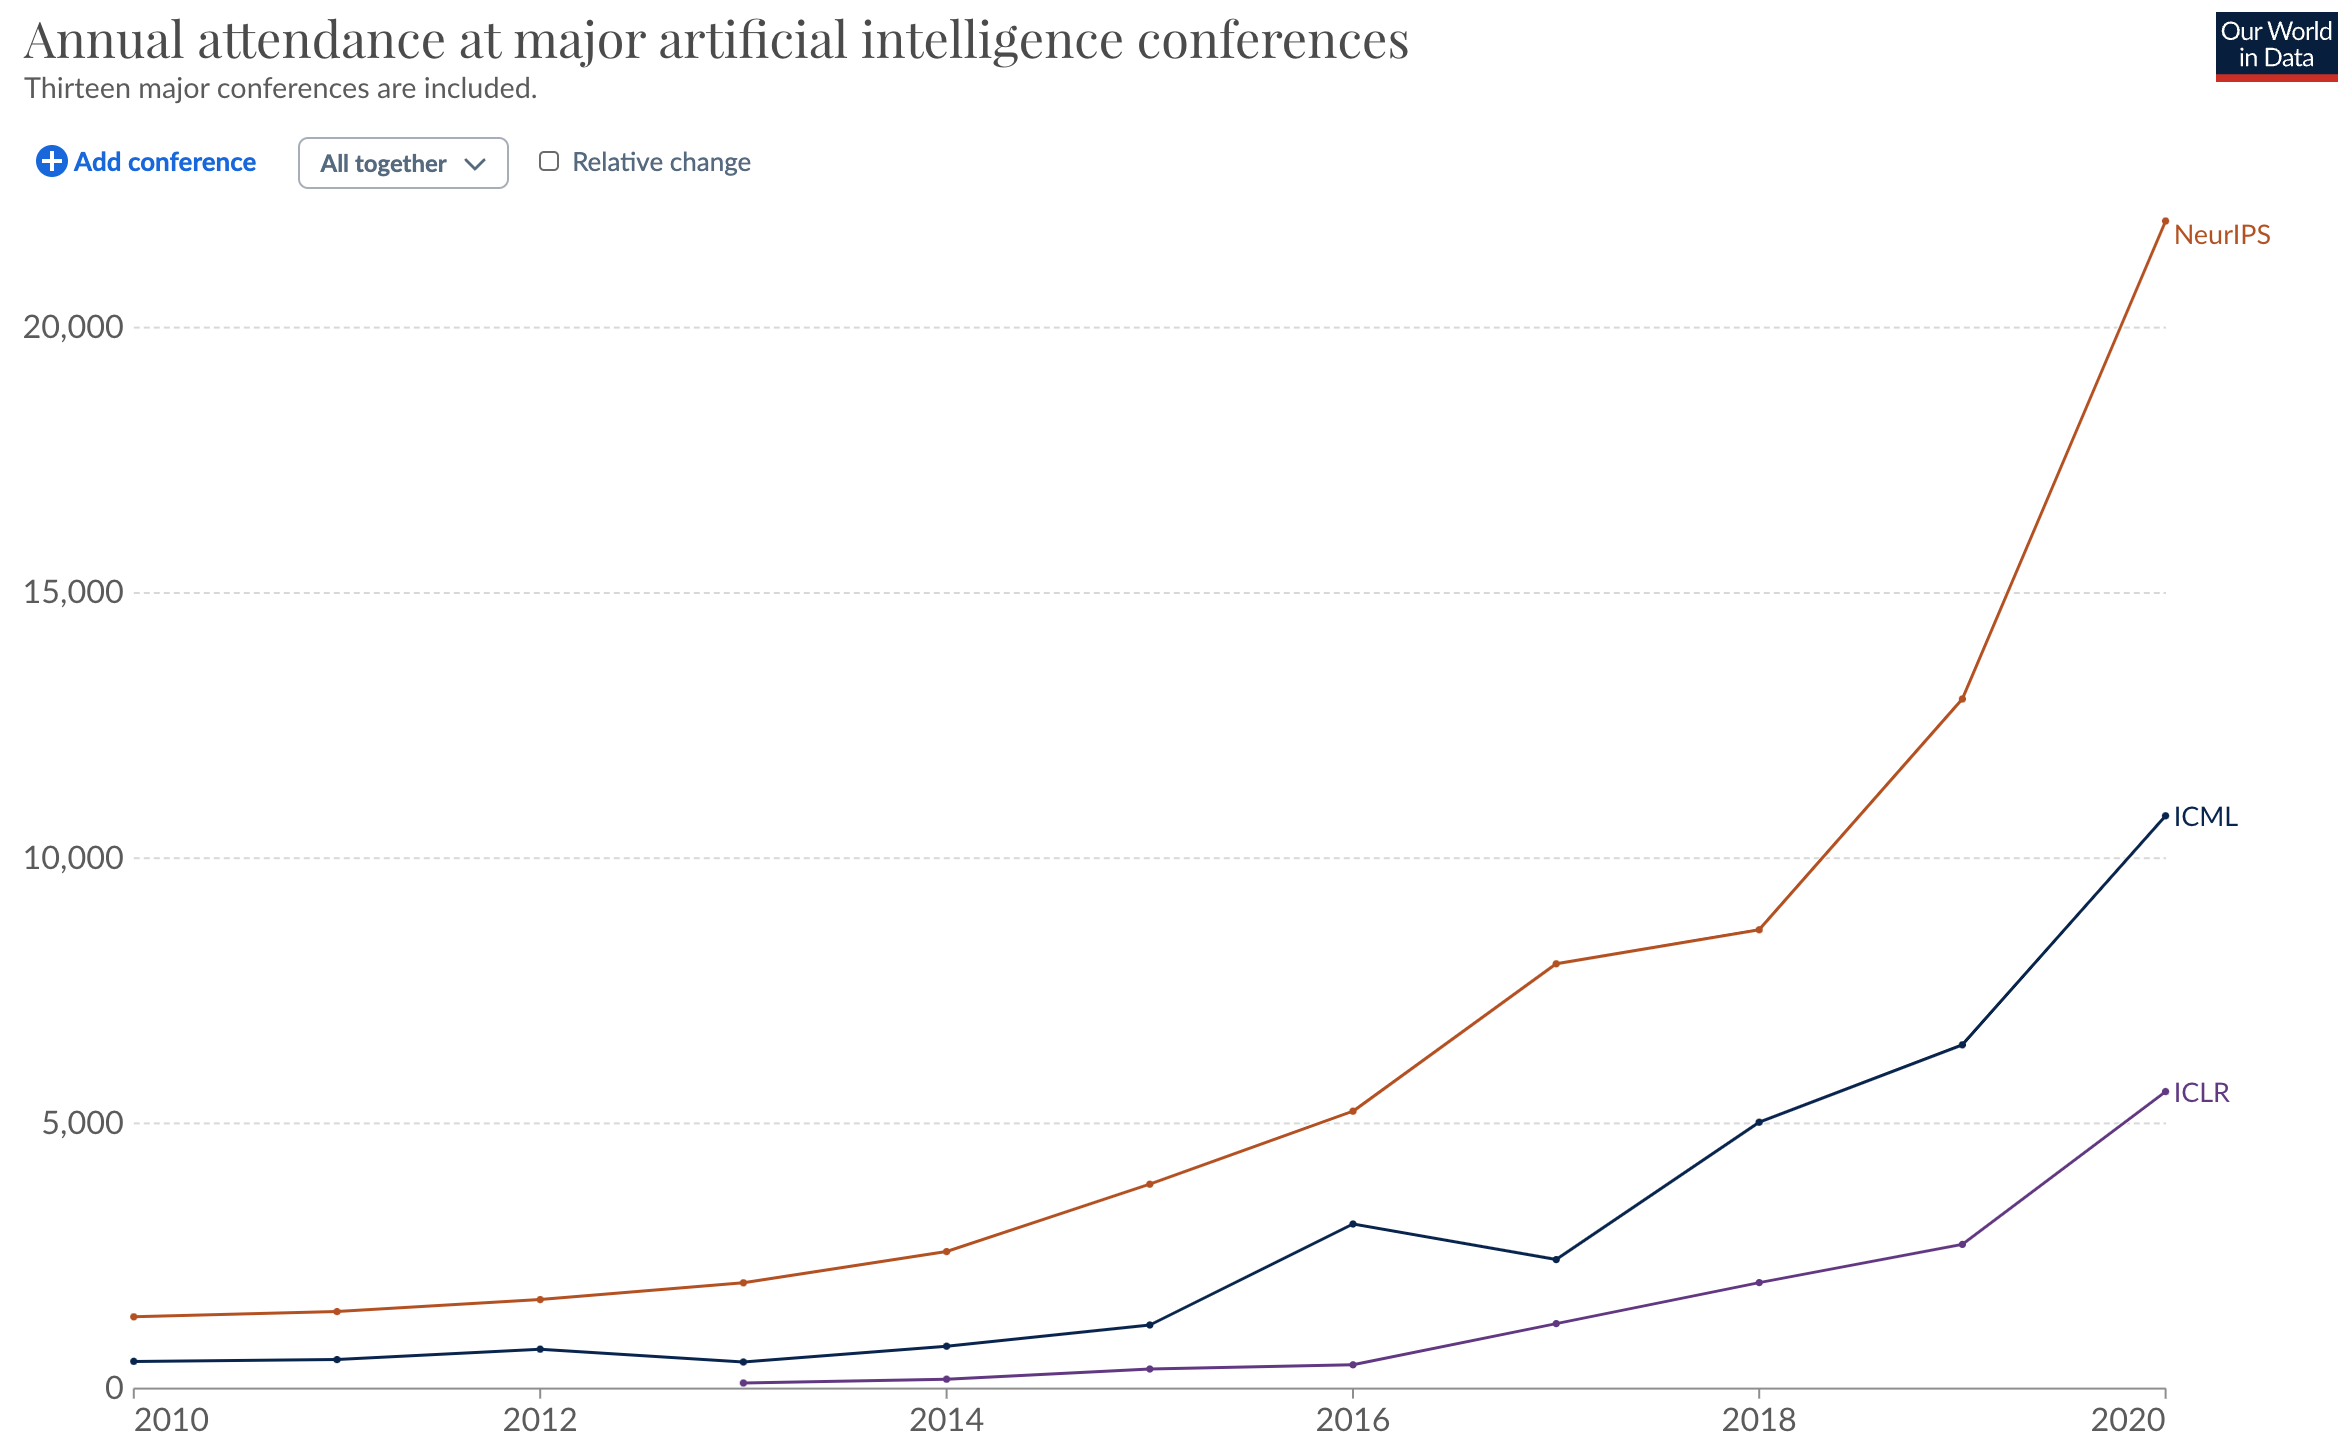
\includegraphics[width=0.7 \linewidth,trim={0 0 0 3.5cm},clip]{figures/attendance.png}
  \end{center}
\end{frame}

\section{Supervised Learning Setup}

\begin{frame}{ML problems}

% \begin{itemize}
% \item 
In supervised learning problems, we generally need to:
\begin{itemize}
    \item<1-> Make a decision:
        \begin{itemize}
            \item Move email to spam folder?
        \end{itemize}
    \item<2-> Take an action:
        \begin{itemize}
            \item In a self-driving car, make a right turn
            \item Reject the hypothesis that $\theta=0$ (classical statistics)
        \end{itemize}
    \item<3-> Produce some output:
        \begin{itemize}
            \item Whose face is it in the image?
            \item The Hindi translation of a Japanese input sentence
        \end{itemize}
    \item<4-> Predicting where a storm will be in an hour (what forms of output are possible here?)
    % \item<5-> An \textbf{action} is the generic term for what is produced by our system.
% \end{itemize}
\end{itemize}

\end{frame}


\begin{frame}{Outcome}
Inputs are often paired with \textbf{labels}.
\begin{exampleblock}{Examples of labels}
\begin{itemize}
\item Whether or not the picture actually contains an animal
\item The storm's location one hour after they query
\item Which, if any, of the suggested URLs were selected
\end{itemize}
\end{exampleblock}
\end{frame}

\begin{frame}{Evaluation Criterion}

Finding ``optimal'' outputs, under various definitions of optimality.
\begin{exampleblock}{Examples of Evaluation Criteria}
\begin{itemize}
\item Is the classification correct? 
\item Does the transcription exactly match the spoken words?
    \begin{itemize}
        \item Should we give partial credit (for getting only some of the words right)? How?
    \end{itemize}

\item How far is the storm from the predicted location? (If we're producing a point estimate)
\item How likely is the storm's actual location under the predicted distribution? (If we're doing density prediction)
\end{itemize}

\end{exampleblock}
\end{frame}


\begin{frame}{Typical Sequence of Events}

Many problem domains can be formalized as follows:
\begin{enumerate}
\item Observe input $x$.
\item Predict an output $\hat{y}$.
\item Observe label $y$.
\item Evaluate output in relation to the label.
\end{enumerate}

% \begin{itemize}
% \item Input space: $\cx$
% \item Label space: $\cy$
% \end{itemize}

\end{frame}

\begin{frame}{Formalization}
\begin{block}{Prediction Function}

A \textbf{prediction function } gets input $x\in\cx$ and produces an output $y\in\cy$.

% \[
% % \begin{matrix}f: & \cx & \rightarrow & \cy\\
% & x & \mapsto & f(x)
% \end{matrix}
% \]
\end{block}

\vspace{2cm}
\begin{block}<2->{Loss Function}

A \textbf{loss function} evaluates the output $\hat{y}$ in the context of the true outcome $y$.
% \[
% \begin{matrix}\loss: & \cy\times\cy & \rightarrow & \reals\\
% & (\hat{y},y) & \mapsto & \loss(\hat{y},y)
% \end{matrix}
% \]
\end{block}
\end{frame}

\begin{frame}{Evaluating a Prediction Function}
    \head{Goal}: Find the optimal prediction function.

    \head{Intuition}: If we can evaluate how good a prediction function is, we can turn this into an optimization problem.

\pause
\begin{itemize}
    \item The loss function $\ell$ evaluates a \emph{single} output
    \item How do we evaluate the prediction function \emph{as a whole}?
\end{itemize}

\end{frame}


\begin{frame}{Loss Function}
Define a space where the prediction function is applicable
\begin{itemize}
\item Assume there is a \textbf{data generating distribution }$P_{\cx\times\cy}.$
\item All input/output pairs $\left(x,y\right)$ are generated i.i.d. from
$P_{\cx\times\cy}.$ 
\end{itemize}

\pause
One common desideratum is to have a prediction function $f(x)$ that ``does well on average'':
\[
\ell(f(x),y)\mbox{ is usually small, in some sense}
\]

How can we formalize this?

\end{frame}
\mode<article>{How can we do time series if we require the examples to be iid? Well
- we have think very carefully about these situations. Usually you
try to reframe the inputs (e.g. by featurization) and outputs so they
seem as iid as possible. }

\begin{frame}{Risk}
\begin{definition}
The \textbf{risk} of a prediction function $f:\cx\to\cy$ is
\[
    R(f)=\ex_{(x,y)\sim P_{\cx\times\cy}}\pb{\loss(f(x),y)}.
\]
In words, it's the \textbf{expected loss} of $f$ over $P_{\cx\times\cy}$.
\end{definition}

% \begin{alertblock}
% {We can't actually compute the risk function:}

\begin{itemize}
\item Since we don't know $P_{\cx\times\cy}$, we cannot compute the expectation.\\

\pause
\item But we can \textbf{estimate} it.
\end{itemize}
% \end{alertblock}
\end{frame}

\begin{frame}{The Bayes Prediction Function }
\begin{definition}
A \textbf{Bayes prediction function} $\minimizer f:\cx\to\cy$ is
a function that achieves the \emph{minimal risk} among all possible
functions: 
\[
\minimizer f\in\argmin_{f}R(f),
\]
where the minimum is taken over all functions from $\cx$ to $\cy$. 
\end{definition}


\begin{itemize}
\item The risk of a Bayes prediction function is called the \textbf{Bayes
risk}.
\item A Bayes prediction function is often called the ``\textbf{target
function}'', since it's the best prediction function we can possibly
produce.
\end{itemize}
\end{frame}

\begin{frame}{Example: Multiclass Classification}
\begin{itemize}
\item Spaces: $\cy=\left\{ 1,\ldots,k\right\} $
\item 0-1 loss: 
\[
\loss(\hat{y},y)=\ind{\hat{y}\neq y}:=\begin{cases}
1 & \mbox{if }\hat{y}\neq y\\
0 & \mbox{otherwise}.
\end{cases}
\]
\end{itemize}

\pause{}
\begin{itemize}
\item Risk: 
\begin{eqnarray*}
R(f) & = & \ex\left[\ind{f(x)\neq y}\right] \quad=0\cdot\pr\left(f(x)=y\right)+1\cdot\pr\left(f(x)\neq y\right)\\
& = & \pr\left(f(x)\neq y\right),
\end{eqnarray*}
which is just the misclassification error rate.

\item The Bayes prediction function returns the most likely
class: 
\[
f^{*}(x)\in\argmax_{1\le c\le k}\pr(y=c\mid x)
\]
\end{itemize}
\end{frame}

\begin{frame}{But we can't compute the risk!}

\begin{itemize}
    \item Can't compute $R(f)=\ex\pb{\loss(f(x),y)}$ because we \textbf{don't know
$P_{\cx\times\cy}$}.

\pause{}
\item One thing we can do in ML/statistics/data science is \textbf{estimate} it:

\pause{}
\begin{block}{Assume we have sample data:}

Let $\cd_{n}=\left((x_{1},y_{1}),\ldots,(x_{n},y_{n})\right)$ be
drawn i.i.d. from $\cp_{\cx\times\cy}$.
\end{block}

\pause{}
\item We draw inspiration from the strong law of large numbers:

If $z_{1},\ldots,z_{n}$ are i.i.d. with expected value $\ex z$,
then
\[
\lim_{n\to\infty}\frac{1}{n}\sum_{i=1}^{n}z_{i}=\ex z,
\]
with probability 1. 
\end{itemize}
\end{frame}

\begin{frame}{The Empirical Risk}

Let $\cd_{n}=\left((x_{1},y_{1}),\ldots,(x_{n},y_{n})\right)$ be
drawn i.i.d. from $\cp_{\cx\times\cy}$.
\begin{definition}
The \textbf{empirical risk}\emph{ }of $f:\cx\to\cy$ with respect
to $\cd_{n}$ is
\[
\hat{R}_{n}(f)=\frac{1}{n}\sum_{i=1}^{n}\loss(f(x_{i}),y_{i}).
\]
\end{definition}

%\begin{itemize}
By the strong law of large numbers, 
\[
\lim_{n\to\infty}\hat{R}_{n}(f)=R(f),
\]
almost surely.


%\item But we want to find the $f$ that \textbf{minimizes} $R(f)$ - will
%minimizing $\hat{R}_{n}(f)$ be good enough?
%\end{itemize}
\end{frame}

\begin{frame}{Empirical Risk Minimization}

\begin{definition}
A function $\hat{f}$ is an \textbf{empirical risk minimizer} if
\[
\hat{f}\in\argmin_{f}\hat{R}_{n}(f),
\]
where the minimum is taken over all functions $f:\cx\to\cy$.
\end{definition}

\begin{itemize}
    \item In an ideal world we'd want to find the risk minimizer.
    \item Is the empirical risk minimizer close enough?
    \item In practice, we always only have a finite sample...
\end{itemize}

\end{frame}

\begin{frame}{Empirical Risk Minimization}

    \begin{itemize}
        \item $P_{\cx}=\mbox{Uniform}[0,1]$, $Y\equiv1$ (i.e. $Y$ is always $1$).

        \item A plot of $\cp_{\cx\times\cy}$:
    \end{itemize}

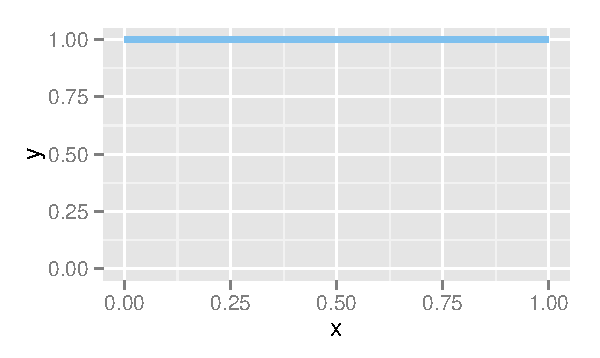
\includegraphics{figures/ERMoverfitting/constantFn} 


\end{frame}

\begin{frame}{Empirical Risk Minimization}

$P_{\cx}=\mbox{Uniform}[0,1]$, $Y\equiv1$ (i.e. $Y$ is always $1$).

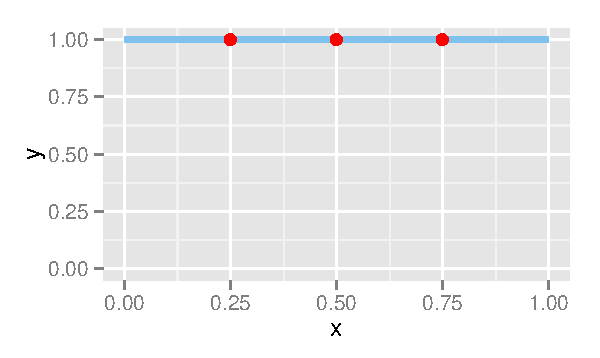
\includegraphics{figures/ERMoverfitting/trainDataConstFn} 

A sample of size $3$ from $\cp_{\cx\times\cy}$.
\end{frame}

\begin{frame}{Empirical Risk Minimization}

$P_{\cx}=\mbox{Uniform}[0,1]$, $Y\equiv1$ (i.e. $Y$ is always $1$).
\begin{center}
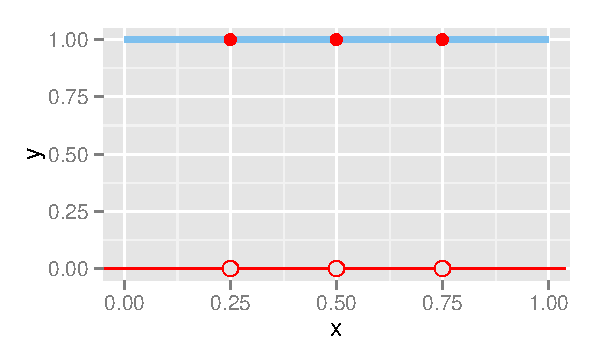
\includegraphics[scale=0.75]{figures/ERMoverfitting/fitAlmostSurely0} 
\par\end{center}

A proposed prediction function:
\[
\hat{f}(x)=\ind{x\in\left\{ 0.25,0.5,0.75\right\} }=\begin{cases}
1 & \mbox{if }x\in\left\{ 0.25,.5,.75\right\} \\
0 & \mbox{otherwise}
\end{cases}
\]

\end{frame}

\begin{frame}{Empirical Risk Minimization}

$P_{\cx}=\mbox{Uniform}[0,1]$, $Y\equiv1$ (i.e. $Y$ is always $1$).

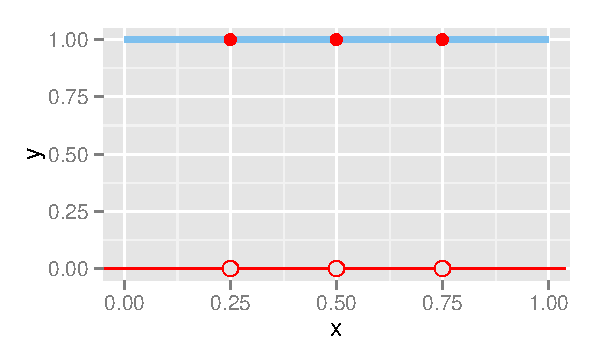
\includegraphics{figures/ERMoverfitting/fitAlmostSurely0} 

Under either the square loss or the 0/1 loss, $\hat{f}$ has Empirical Risk = 0 and
Risk = 1. 
\end{frame}

\begin{frame}{Empirical Risk Minimization}

\begin{itemize}
    \item In this case, ERM led to a function $f$ that just \al{memorized} the data.
\item How can we improve \textbf{generalization} from the training
inputs to new inputs?

\item We need to smooth things out somehow!
\begin{itemize}
\item A lot of modeling is about spreading and extrapolating information
from one part of the input space $\cx$ into unobserved parts of the
space.

\end{itemize}
\item One approach is \textbf{constrained ERM}:

\begin{itemize}
    \item Instead of minimizing empirical risk over \emph{all} prediction functions,
    \item We constrain our search to a particular subset of the space of functions, called a \textbf{hypothesis space}.
\end{itemize}
\end{itemize}
\end{frame}

\begin{frame}{Hypothesis Spaces}
\begin{definition}
A \textbf{hypothesis space} $\cf$ is a set of prediction functions $\cx\to\cy$ that we consider when applying ERM.
\end{definition}

Desirable properties of a hypothesis space:
\begin{itemize}
\item Includes only those functions that have the desired ``regularity'', e.g. smoothness, simplicity
\item Easy to work with (e.g., we have efficient algorithms to find the best function within the space)
\end{itemize}

Most applied work is about designing good hypothesis spaces for specific tasks.
\end{frame}

\begin{frame}{Constrained Empirical Risk Minimization}
\begin{itemize}
\item Given a hypothesis space $\cf$, a set of prediction functions mapping
$\cx\to\cy$,
\item An \textbf{empirical risk minimizer }(ERM) in $\cf$ is a function $\hat{f}_{n}$ such that
\[
    \hat{f}_{n}\in\argmin_{\hl{f\in\cf}}\frac{1}{n}\sum_{i=1}^{n}\loss(f(x_{i}),y_{i}).
\]

\item A \textbf{risk minimizer }in $\cf$ is a function $\minimizer{f_{\cf}}\in\cf$ such that
\[
    \minimizer{f_{\cf}}\in\argmin_{\hl{f\in\cf}}\ex\pb{\loss(f(x),y)}.
\]
\end{itemize}
\end{frame}

\mode<article>{The hat on $f$ in $\hat{f}_{n}$ indicates that $\hat{f}_{n}$ depends
on the sample data. The subscript $n$ just designates that the sample
was of size $n$.} 

\begin{frame}{Excess Risk Decomposition}
\begin{columns}[c]

\column{.4\textwidth}

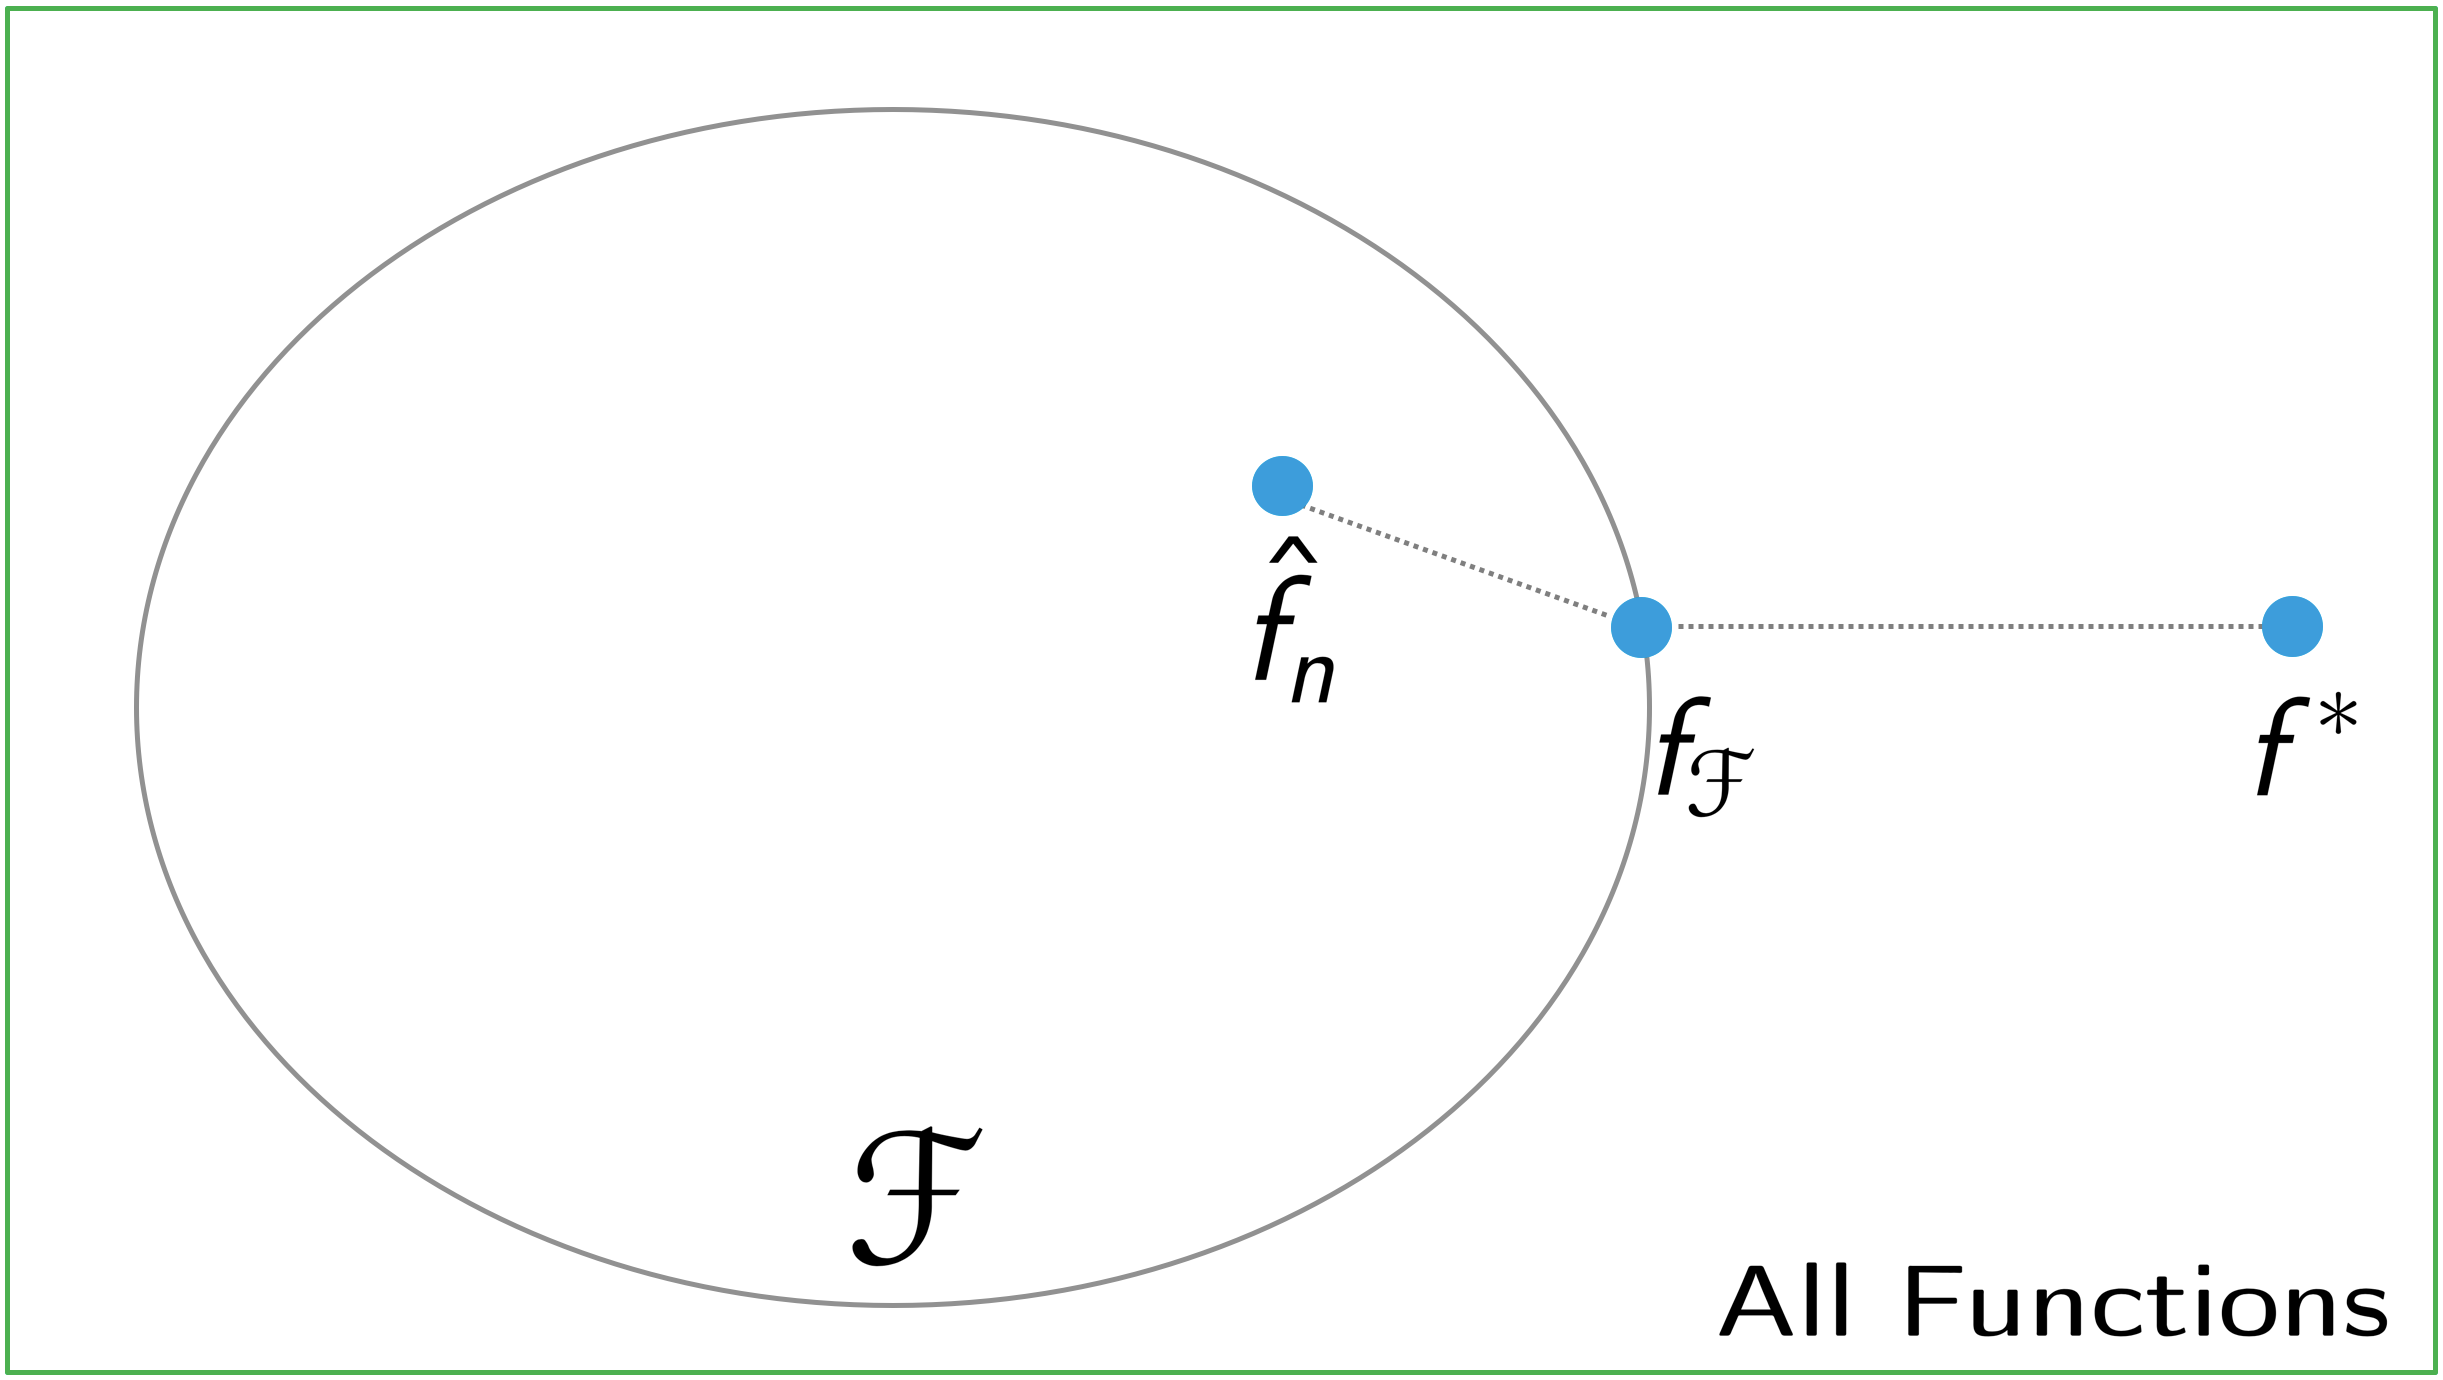
\includegraphics[width=1\columnwidth]{figures/error-decomp}

\column{.4\textwidth}

\begin{align*}
    f^{*}= & \argmin_{f}\ex\pb{\ell(f(x),y)}\\
    f_{\cf}= & \argmin_{f\in\cf}\ex\pb{\ell(f(x),y)}\\
\hat{f}_{n}= & \argmin_{f\in\cf}\frac{1}{n}\sum_{i=1}^{n}\ell(f(x_{i}),y_{i})
\end{align*}
\end{columns}


\begin{itemize}
\item \textbf{Approximation error }(of $\cf$)\textbf{ $=\ R(f_{\cf})-R(\minimizer f)$}
\item \textbf{Estimation error} (of $\hat{f}_{n}$ in $\cf$) $=\ R(\hat{f}_{n})-R(f_{\cf})$ 
\end{itemize}
\end{frame}
\mode<article>{This diagram shows the space of all functions. The hypothesis space
$\cf$ carves out a subset of that space. The Bayes prediction function
$f^{*}$ will not typically be contained in $\cf$. The best we can
possibly do in terms of risk (i.e. the expected loss on a new randomly
chosen data point), which is our ultimate performance measure, is
$f_{\cf}$. How much worse does $f_{\cf}$ perform than $f^{*}$?
That's our potential penalty for restricting to a hypothesis space
$\cf$. We hope it will be more than compensated by reduction in overfitting.
We can write down that performance gap explicitly, and it's called
approximation error. (Parenthetically, Approximation theory is a field
of mathematics that studies how well one can approximate a function
by simpler functions -- e.g. using polynomials, or sins and cosines
or wavelets to approximate a given function. And studying how well
these approximations work.) Approximation error of a hypothesis space
$\cf$ is $\risk(f_{\cf})-\risk(f^{*})$. 

Concept checks: 1) Can approximation error be negative?

2) Is approximation a random quantity?

Now, of course we cannot find $f_{\cf}$, since we can't evaluate
the true risk $\risk$. So in practice, we work with the empirical
risk $\hat{R}$ based on sample of data, a training set. We find the
empirical risk minimizer $\hat{f}_{n}$ in the hypothesis space $\cf$. }

\begin{frame}{Approximation Error}

Approximation error $\risk(f_{\cf})-\risk(\minimizer f)$ is
\begin{itemize}
\item a property of the class $\cf$

\item the penalty for restricting to $\cf$ (rather than considering all
possible functions)
\end{itemize}


\emph{Bigger} $\cf$ mean \emph{smaller }approximation error. 

Concept check: Is approximation error a random or non-random variable?
\end{frame}

\begin{frame}{Estimation Error}

Estimation error $\risk(\hat{f}_{n})-\risk(f_{\cf})$
\begin{itemize}
\item is the performance hit for choosing $f$ using finite training data

\item is the performance hit for minimizing empirical risk rather than true
risk 
\end{itemize}

With\emph{ smaller }$\cf$ we expect \emph{smaller }estimation error.

\emph{Under typical conditions: ``}With infinite training data, estimation
error goes to zero.''

Concept check: Is estimation error a random or non-random variable?
\end{frame}

% \begin{frame}{Excess Risk Decomposition for ERM}
% \begin{definition}
% The \textbf{excess risk} compares the risk of $f$ to the Bayes optimal
% $f^{*}$:
% \[
% \mbox{\textbf{Excess Risk}}(f)\,=\,\risk(f)-\risk(\minimizer f)
% \]
% \end{definition}

% \begin{itemize}
% \item Can excess risk ever be negative? 
% \end{itemize}

% The excess risk of the ERM $\hat{f}_{n}$ can be decomposed:
% \begin{eqnarray*}
% \mbox{\textbf{Excess Risk}}(\hat{f}_{n}) & = & \risk(\hat{f}_{n})-\risk(\minimizer f)\\
% & = & \underbrace{\risk(\hat{f}_{n})-\risk(f_{\cf})}_{\text{estimation error}}+\underbrace{\risk(f_{\cf})-\risk(\minimizer f)}_{\text{approximation error}}.
% \end{eqnarray*}
% \begin{itemize}
% \item There is a tradeoff between estimation error and approximation error
% \end{itemize}
% \end{frame}

\begin{frame}{ERM in Practice}
\begin{itemize}
\item<1-> What have we been glossing over by writing ``argmin''?

\item<2-> In practice, we need a method to find $\hat{f}_{n}\in\cf$: this can be very difficult!

\item<3-> For nice choices of loss functions and classes $\cf$, we can get
arbitrarily close to the exact minimizer
\begin{itemize}
\item But that takes time -- is it always worth it?
\end{itemize}
\item<4-> For some hypothesis spaces (e.g. neural networks), we don't know how
to find $\hat{f}_{n}\in\cf$. 
\end{itemize}
\end{frame}

\begin{frame}{Optimization Error}
\begin{itemize}
\item In practice, we don't find the ERM $\hat{f}_{n}\in\cf$. 
\item We find $\tilde{f}_{n}\in\cf$ that we hope is good enough.
\item \textbf{Optimization error: }If $\tilde{f}_{n}$ is the function our
optimization method returns, and $\hat{f}_{n}$ is the empirical risk
minimizer, then
\[
\mbox{Optimization Error }=\;R(\tilde{f}_{n})-R(\hat{f}_{n}).
\]
 

%\item Can optimization error be negative? Yes!
%\item But
%\[
%\hat{R}(\tilde{f}_{n})-\hat{R}(\hat{f}_{n})\ge0.
%\]
 
\end{itemize}
\end{frame}

\begin{frame}{Error Decomposition in Practice}
\begin{itemize}
\item Excess risk decomposition for function $\tilde{f}_{n}$ returned by
an optimization algorithm in practice:
\begin{align*}
\mbox{\textbf{Excess Risk}}(\tilde{f}_{n})\, & =\,\risk(\tilde{f}_{n})-\risk(\minimizer f)\\
 & =\underbrace{\risk(\tilde{f}_{n})-R(\hat{f}_{n})}_{\text{optimization error}}+\underbrace{\risk(\hat{f}_{n})-\risk(f_{\cf})}_{\text{estimation error}}+\underbrace{\risk(f_{\cf})-\risk(\minimizer f)}_{\text{approximation error}}
\end{align*}


% \item It would be nice to observe the error decomposition for a practical $\tilde{f}_{n}$!
\item How would we address each type of error?
% \item Why is this usually impossible?

% \item But we could constuct an artificial example, where we know $P_{\cx\times\cy}$
% and $f^{*}$ and $f_{\cf}$...
\end{itemize}
\end{frame}

\begin{frame}{ERM Overview}
\begin{itemize}
\item<1-> Given a loss function $\loss$,
\item<2-> Choose a hypothesis space $\cf$.
\item<3-> Use an optimization method to find an empirical risk minimizer $\hat{f}_{n}\in\cf$:
\[
\hat{f}_{n}=\argmin_{f\in\cf}\frac{1}{n}\sum_{i=1}^{n}\loss(f(x_{i}),y_{i}).
\]
\item<4-> Or find a $\tilde{f}_{n}$ that comes close to $\hat{f}_{n}$
\item<5-> The machine learning scientist's job: 
\begin{itemize}
\item Choose $\cf$ that balances approximation and estimation error.
\item As we get more training data, we can use a bigger $\cf$.
\end{itemize}
\end{itemize}
\end{frame}

\end{document}
